\documentclass[11pt,titlepage]{article}

%Laenderspezifische Einstellungen bzgl. Rechtschreibung, Sonderzeichen und Kodierung
\usepackage[utf8]{inputenc}
\usepackage[english]{babel}
\usepackage[T1]{fontenc}
\usepackage{titlesec}
\usepackage{graphicx}
%\usepackage{subcaption}

\usepackage{listings}
\usepackage{color}
\usepackage{courier}
\definecolor{light-gray}{gray}{0.85}
\lstset{
language=C++,
numbers=left,
breaklines=true,
backgroundcolor=\color{light-gray},
tabsize=2,
basicstyle=\footnotesize\ttfamily,
frame=single,
inputencoding=utf8,
extendedchars=true,
showstringspaces=false,
literate =
	{ä}{{\"a}}1
	{ö}{{\"o}}1
	{ü}{{\"u}}1
	{Ä}{{\"A}}1
	{Ö}{{\"O}}1
	{Ü}{{\"U}}1
	{ß}{{\ss}}1
	{ₙ}{{$_n$}}1
}

\def\ContinueLineNumber{\lstset{firstnumber=last}}
\def\StartLineAt#1{\lstset{firstnumber=#1}}

\usepackage[
	a4paper,
	top = 2cm,
	bottom = 2 cm,
	left = 2cm,
	right = 2cm,
	headheight = 15pt,
	includeheadfoot
	]{geometry}
\usepackage{fancyhdr}
\usepackage{amssymb}
\usepackage{amsmath}
\usepackage[english]{varioref}
\usepackage{hyperref}

\fancypagestyle{fancy}{
	\fancyhead[R]{Page \thepage}
	\fancyhead[L]{\leftmark}
	\renewcommand{\headrulewidth}{1.25pt}

	\fancyfoot[L]{\tiny{Programming 2 - Assignment 2, created: \today}}
	\fancyfoot[R]{\tiny{ Felix Dreßler (k12105003)}}
	\cfoot{}
	\renewcommand{\footrulewidth}{1.25pt}
}

\setlength{\headsep}{10mm}
\setlength{\footskip}{10mm}

\setlength{\parindent}{0mm}
\setlength{\parskip}{1.1ex plus0.25ex minus0.25ex}
\setlength{\tabcolsep}{0.2cm} % for the horizontal padding

\pagestyle{fancy}

\title{Programming 2 - Assignment 2}
\author{Felix Dreßler (k12105003)\\ email \href{mailto:FelixDressler01@gmail.com}{FelixDressler01@gmail.com}}
\date{\today} %Erstellungsdatum

\begin{document}
\maketitle
	\section{Testing the Program}
	For testing the Program, or in specific, the class, a series of tests was performed by testing different methods of this through different main-methods.
	
	\subsection{testing the specified commands}
	In this section the commands given in the assignment instructions will be tested.
	
	The following code-block shows the methods used to perform the first test. As shown, every operation was performed in two variables, with multiple inclusions of both \emph{add()} methods and the \emph{println()} method.
		\lstinputlisting[]{Documentation/Main/Main.cpp}
		
	This is the output, that was created by the code above.
		\lstinputlisting[numbers=none]{Documentation/Main/test-output.txt}
		
\newpage	
	\subsection{testing in three and one variable}
	In this section, tests of the class in one and three variables will be presented. In order to produce results that are comparable we modified the test case from the previous section to work with uni- and three-variate polynomials.
	By modifying it further, adding zero-polynomials was also tested.
	
		\subsubsection{testing in one variable}
		The following code was used to perform the tests.
			\lstinputlisting[]{Documentation/specific_tests/Main3.cpp}
\newpage	
		This is the output, that was created by the code above.
			\lstinputlisting[numbers=none]{Documentation/specific_tests/test-output3.txt}
		
		\subsubsection{testing in three variables}
		The following code was used to perform the tests.
			\lstinputlisting[]{Documentation/specific_tests/Main1.cpp}
			
		This is the output, that was created by the code above.
			\lstinputlisting[numbers=none]{Documentation/specific_tests/test-output1.txt}
\newpage			
		\subsubsection{adding the zero-polynomial}
		The following code was used to perform the tests.
			\lstinputlisting[]{Documentation/specific_tests/Main2.cpp}
		
		This is the output, that was created by the code above.
			\lstinputlisting[numbers=none]{Documentation/specific_tests/test-output2.txt}
			
\newpage		
	\subsection{testing error messages}
	In this section, we will test different kinds of errors that can occur during programming with this class.
	We will try to produce error messages.
	
		\subsubsection{adding polynomials with different numbers of variables}
		The following code was used to perform the tests.
			\lstinputlisting[]{Documentation/Errors/Main1.cpp}
		
		This is the output, that was created by the code above. The desired error message has been printed successfully.
			\lstinputlisting[numbers=none]{Documentation/Errors/Error1.txt}
			
		\subsubsection{adding polynomials with different orders of variables}
		The following code was used to perform the tests.
			\lstinputlisting[]{Documentation/Errors/Main2.cpp}
		
		This is the output, that was created by the code above. The desired error message has been printed successfully.
			\lstinputlisting[numbers=none]{Documentation/Errors/Error2.txt}
\newpage

		
	\section{Problems}
	This section will briefly discuss the Problems that have occurred during programming.
		\subsection{warnings}
		In the \emph{resize} method, line 283 of the \emph{DistPoly.cpp} this warning is displayed:
		
			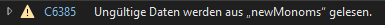
\includegraphics[scale=1.5]{Documentation/warning-line297.png}
		
		\StartLineAt{281}	
		\lstinputlisting[linerange={279-292}]{Assignment2/Assignment2/DistPoly.cpp}
		
		This is probably caused in connection by the copy assignment operator of the \emph{Monom} class, because as soon as we disable all methods of the \emph{Monom} class, this warning disappears.
		
	
\newpage
		
	\section{The Class - DistPoly.h}
	This section shows the Header file in which the \emph{DistPoly} class is defined.
	
		\lstinputlisting[]{Assignment2/Assignment2/DistPoly.h}
	
\newpage
	\section{The Class - DistPoly.cpp}
		This section shows the .cpp file in which the \emph{DistPoly} class is implemented.
		
		Note: The copy constructor could also be implemented by using the add function.	
		
		\lstinputlisting[]{Assignment2/Assignment2/DistPoly.cpp}	

\end{document}